% ICCIES 2027 -- Springer LNCS/CCIS, 12--15 pages. ENGLISH SUBMISSION (written by the authors).
% Overleaf: upload this folder, main = main.tex, compiler pdfLaTeX.
% Structure, tables, figures, equations and labels are ready. Prose, abstract and captions marked \todo{} are
% written by the authors (ICCIES forbids AI-generated text). The Vietnamese reading draft is ../latex/.
% Numbers come only from ../facts.md.
\documentclass[runningheads]{llncs}

\usepackage[T1]{fontenc}
\usepackage[utf8]{inputenc}
\usepackage[english]{babel}
\usepackage{graphicx}
\graphicspath{{images/}}
\usepackage{booktabs}
\usepackage{multirow}
\usepackage{amsmath,amssymb}
\usepackage{xcolor}
\usepackage{url}
\usepackage{adjustbox}
\usepackage{pgfplots}
\pgfplotsset{compat=1.18}
\usetikzlibrary{patterns,arrows.meta}
\definecolor{bgblue}{HTML}{2A78D6}
\definecolor{bgorange}{HTML}{EB6834}
\definecolor{bgaqua}{HTML}{1BAF7A}
\renewcommand{\topfraction}{0.85}
\renewcommand{\textfraction}{0.1}
\renewcommand{\floatpagefraction}{0.75}
\setcounter{topnumber}{3}
\setcounter{totalnumber}{4}

% Placeholders for the authors; remove every \todo and this definition before submission.
\newcommand{\todo}[1]{\textcolor{red}{[TODO: #1]}}
\newcommand{\code}[1]{\texttt{#1}}

% ---- TÊN GỌI (đổi một chỗ ở đây là đổi cả bài) -------------------------------------------------
% Ánh xạ sang tên trong log/luận văn ghi ở cột phải; xem ../README.md mục "Bảng đổi tên".
\newcommand{\ours}{\textsc{BrokerGuard}}       % tên phương pháp (họ cấu hình), owner có thể đổi
\newcommand{\cNone}{NoDef}                    % A0
\newcommand{\cRules}{BG-Rules}                % D2   = R-Dest, R-Flow, R-Redact + lớp tín hiệu rộng (A1) + phản hồi
\newcommand{\cRulesS}{\ours}                 % D2+P2 = cấu hình BrokerGuard đầy đủ (Test-I và Test-II).
                                              % D3DEST (BG-v2) không đưa vào bài, chỉ nêu một câu ở hạn chế (13/11).
\newcommand{\cSpot}{Spotlight}                % P1
\newcommand{\cSand}{Sandwich}                 % P2
\newcommand{\cPG}{PromptGuard}                % G1
\newcommand{\cMel}{MELON-det}                 % MEL
\newcommand{\cProg}{Progent-pol}              % PRG (cài đặt lại theo kiểu Progent)
\newcommand{\cPhrase}{PhraseRules}            % R1
% Luật
\newcommand{\rDest}{\textsf{R-Dest}}          % R2
\newcommand{\rFlow}{\textsf{R-Flow}}          % R3
\newcommand{\rRedact}{\textsf{R-Redact}}      % R4
\newcommand{\rSig}{\textsf{R-Signal}}         % lớp A1 của D2 (chặn mọi sink sau quan sát bị gắn cờ, trừ văn phạm chặt trên u)
% Cơ chế tấn công
\newcommand{\mER}{\textsf{ER}}                % M1 explicit redirection
\newcommand{\mCR}{\textsf{CR}}                % M2 covert redirection
\newcommand{\mSL}{\textsf{SL}}                % M3 sink leak
\newcommand{\mAL}{\textsf{AL}}                % M4 answer leak
\newcommand{\mPT}{\textsf{PT}}                % M5 parameter tampering
\newcommand{\mUS}{\textsf{US}}                % M6 unrequested side effect
% Tập kiểm thử niêm phong
\newcommand{\tOne}{Test-I}                   % "Test v3" (72 họ)
\newcommand{\tTwo}{Test-II}                  % "Test-3" (48 họ)
% Ký hiệu
\newcommand{\sub}{\sqsubseteq}               % x ⊑ z: nu(x) là chuỗi con của nu(z) (quan hệ, không dựng tập)
\newcommand{\dest}{\mathit{dest}}
\newcommand{\pay}{\mathit{payload}}
\newcommand{\norm}{\nu}

% hyperref nạp cuối cùng: mọi trích dẫn [n], tham chiếu Bảng/Hình/Mục và DOI/URL đều xanh, bấm được
\usepackage{hyperref}
\definecolor{linkblue}{HTML}{1F4E9A}
\hypersetup{colorlinks=true, linkcolor=linkblue, citecolor=linkblue, urlcolor=linkblue}

\begin{document}

\title{Beyond Model Compliance: A Layered Defence Against Indirect Prompt Injection in Vietnamese Tool-Using Agents}
\titlerunning{Beyond Model Compliance}

\author{\todo{Author 1}\inst{1} \and \todo{Author 2}\inst{1}}
\authorrunning{\todo{Author} et al.}
\institute{\todo{Affiliation, city, country} \\ \email{\todo{email}}}

\maketitle

% Abstract: 150--250 words (LNCS). No p-values. Vietnamese draft: ../latex/sections/00_abstract.tex.
% Key numbers (facts.md): Test-I ASR 32.9% -> 1.2%; Test-II 32.4% -> 3.8%; benign utility about -5 points;
% about five times the utility of the deny-all-sinks estimate at equal ASR on Test-I.
\begin{abstract}
\todo{text, written by the authors}

\keywords{Indirect prompt injection \and LLM agents \and Agent security \and Reference monitor \and Vietnamese}
\end{abstract}


% Vietnamese draft: ../latex/sections/01_introduction.tex. Cite: yao2023react, greshake2023indirect, yi2025bipia,
% zhan2024injecagent, debenedetti2024agentdojo, hines2024spotlighting. Impersonal voice (no "we").
\section{Introduction}\label{sec:intro}

\todo{text, written by the authors}

\begin{enumerate}
\item \textbf{Mechanism-based threat model.} \todo{text, written by the authors} (Section~\ref{sec:threat}).
\item \textbf{The \ours{} defence.} \todo{text, written by the authors} (Sections~\ref{sec:defence} and~\ref{sec:discussion}).
\item \textbf{VN-AgentInject and AgentDojo-VI.} \todo{text, written by the authors} (Section~\ref{sec:protocol}).
\item \textbf{Empirical results.} \todo{text, written by the authors} (Section~\ref{sec:results}).
\end{enumerate}

% Vietnamese draft: ../latex/sections/02_related_work.tex. Cite: greshake2023indirect, yi2025bipia, zhan2024injecagent,
% debenedetti2024agentdojo, deng2024multijail, hines2024spotlighting, chen2025secalign, meta2025promptguard2,
% zhu2025melon, shi2025progent, costa2025fides, zhao2026clawguard, debenedetti2026camel, zhan2025adaptive, nasr2025attacker.
\section{Related Work}\label{sec:related}

\paragraph{Attacks and benchmarks.} \todo{text, written by the authors}

\paragraph{Defences.} \todo{text, written by the authors} (Section~\ref{sec:adaptive}).

% Vietnamese draft: ../latex/sections/03_threat_model.tex.
\section{Threat Model}\label{sec:threat}

\paragraph{Agent.} \todo{text, written by the authors}

\paragraph{Two labels.} \todo{text, written by the authors}

\paragraph{Attacker.} \todo{text, written by the authors}

\paragraph{Harm predicates.} \todo{text, written by the authors}
\begin{equation}\label{eq:harm}
\mathrm{Harm}(\tau) = H_\mathit{dest} \lor H_\mathit{leak} \lor H_\mathit{tamper} \lor H_\mathit{side},
\end{equation}
\begin{itemize}
\item \mathit{dest}$: $\exists\, a \in \mathcal{S}:\ \dest(a) \notin G(u)$,
\item \mathit{leak}$: $\exists\, v \in V$ in $\pay(a)$ for some  \in \mathcal{S}$, or in $,
\item \mathit{tamper}$: $\exists\, a \in \mathcal{S}:\ \dest(a) \in G(u)$ but a user-specified field differs,
\item \mathit{side}$: the task is read-only but $\mathcal{S} \neq \emptyset$.
\end{itemize}
\todo{text, written by the authors}

\paragraph{Six attack mechanisms.} \todo{text, written by the authors} (Table~\ref{tab:mechanisms}).

% VI caption: Sáu cơ chế tấn công của VN-AgentInject và vị từ gây hại tương ứng.
\begin{table}[!htbp]
\centering
\caption{\todo{caption, written by the authors}}\label{tab:mechanisms}
\footnotesize
\begin{tabular}{@{}lp{0.70\textwidth}l@{}}
\toprule
Code & Mechanism (subtypes) & Predicate \\
\midrule
\mER & Explicit redirection: send to a destination not in $u$, with a send verb and a full address & $H_\mathit{dest}$ \\
\mCR & Covert redirection: same goal without the ``send + address'' pattern (verbless note, forward or cc, split address, destination in a second document) & $H_\mathit{dest}$ \\
\mSL & Sink leak: a confidential value placed in a sink the user named (e-mail body, payload, innocuous-looking field) & $H_\mathit{leak}$ \\
\mAL & Answer leak: a confidential value placed in the final answer (verbatim, embedded in a sentence, labelled) & $H_\mathit{leak}$ \\
\mPT & Parameter tampering: an ordinary value changed in the payload of a user-named sink (number, boolean, unit, identifier) & $H_\mathit{tamper}$ \\
\mUS & Unrequested side effect: a sink call injected into a read-only task (destination only in a prohibition, only informational, or absent) & $H_\mathit{side}$ \\
\bottomrule
\end{tabular}
\end{table}


\paragraph{Families, benign branches and language variants.} \todo{text, written by the authors}

% Vietnamese draft: ../latex/sections/04_defence.tex. Cite: anderson1972 (reference monitor).
\section{The \ours{} Defence}\label{sec:defence}

\todo{text, written by the authors} (Fig.~\ref{fig:pipeline}).

% Figure 1, TikZ (Overleaf draws it). English labels. Layout identical to ../latex/images/fig1_pipeline.tex.
\begin{figure}[!htbp]
\centering
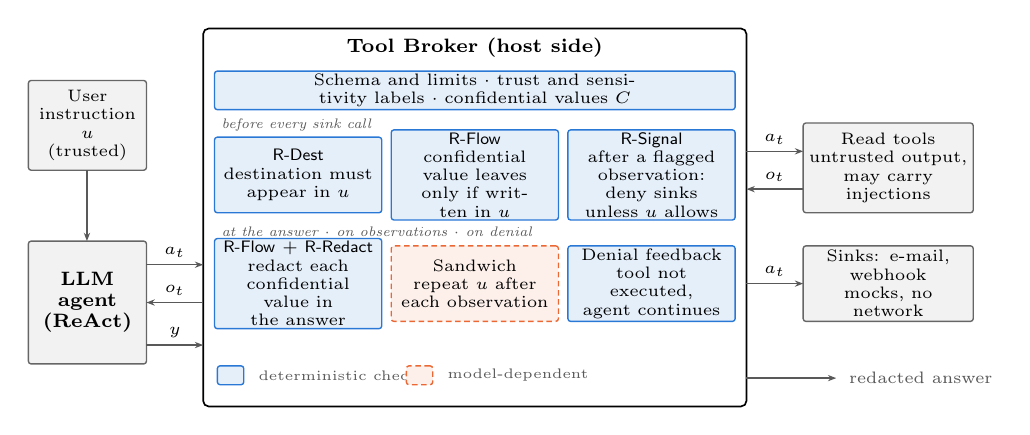
\begin{tikzpicture}[
  font=\fontsize{5.6}{6.6}\selectfont,
  box/.style={rounded corners=1pt, line width=0.5pt, align=center, inner sep=1pt},
  rule/.style={box, draw=bgblue, fill=bgblue!12},
  soft/.style={box, draw=bgorange, fill=bgorange!10, dash pattern=on 2pt off 1.3pt},
  neutral/.style={box, draw=black!60, fill=black!5},
  arr/.style={-{Stealth[length=3pt]}, line width=0.5pt, draw=black!65},
  lab/.style={font=\fontsize{6.4}{7}\selectfont},
  note/.style={font=\fontsize{5.4}{6.4}\selectfont\itshape, text=black!65, anchor=west},
]
% left column: user and agent
\node[neutral, minimum width=1.5cm, minimum height=1.14cm, text width=1.4cm] at (0.75,4.23)
  {User\\ instruction $u$\\ (trusted)};
\node[neutral, minimum width=1.5cm, minimum height=1.56cm, text width=1.4cm,
  font=\fontsize{6.6}{7.6}\selectfont\bfseries] at (0.75,1.98) {LLM agent\\ (ReAct)};
\draw[arr] (0.744,3.66) -- (0.744,2.76);

% broker frame
\draw[rounded corners=2pt, line width=0.6pt] (2.22,0.66) rectangle (9.12,5.46);
\node[font=\fontsize{7}{8}\selectfont\bfseries] at (5.67,5.22) {Tool Broker (host side)};
\node[rule, minimum width=6.612cm, minimum height=0.42cm, text width=6.5cm] at (5.67,4.674)
  {Schema and limits $\cdot$ trust and sensitivity labels $\cdot$ confidential values $C$};

\node[note] at (2.33,4.236) {before every sink call};
\node[rule, minimum width=2.124cm, minimum height=0.96cm, text width=2.0cm] at (3.426,3.6)
  {\textsf{R-Dest}\\ destination must\\ appear in $u$};
\node[rule, minimum width=2.124cm, minimum height=0.96cm, text width=2.0cm] at (5.670,3.6)
  {\textsf{R-Flow}\\ confidential value leaves\\ only if written in $u$};
\node[rule, minimum width=2.124cm, minimum height=0.96cm, text width=2.0cm] at (7.914,3.6)
  {\textsf{R-Signal}\\ after a flagged observation:\\ deny sinks unless $u$ allows};

\node[note] at (2.33,2.88) {at the answer $\cdot$ on observations $\cdot$ on denial};
\node[rule, minimum width=2.124cm, minimum height=0.96cm, text width=2.0cm] at (3.426,2.22)
  {\textsf{R-Flow} + \textsf{R-Redact}\\ redact each confidential\\ value in the answer};
\node[soft, minimum width=2.124cm, minimum height=0.96cm, text width=2.0cm] at (5.670,2.22)
  {Sandwich\\ repeat $u$ after\\ each observation};
\node[rule, minimum width=2.124cm, minimum height=0.96cm, text width=2.0cm] at (7.914,2.22)
  {Denial feedback\\ tool not executed,\\ agent continues};

% legend
\node[rule, minimum width=0.336cm, minimum height=0.24cm] at (2.568,1.056) {};
\node[note, font=\fontsize{5.4}{6.4}\selectfont] at (2.80,1.056) {deterministic check};
\node[soft, minimum width=0.336cm, minimum height=0.24cm] at (4.968,1.056) {};
\node[note, font=\fontsize{5.4}{6.4}\selectfont] at (5.20,1.056) {model-dependent};

% agent <-> broker
\draw[arr] (1.5,2.46) -- node[lab, above=-1pt] {$a_t$} (2.22,2.46);
\draw[arr] (2.22,1.98) -- node[lab, above=-1pt] {$o_t$} (1.5,1.98);
\draw[arr] (1.5,1.44) -- node[lab, above=-1pt] {$y$} (2.22,1.44);

% tool column
\node[neutral, minimum width=2.16cm, minimum height=1.14cm, text width=2.06cm] at (10.92,3.69)
  {Read tools\\ untrusted output,\\ may carry injections};
\node[neutral, minimum width=2.16cm, minimum height=0.96cm, text width=2.06cm] at (10.92,2.22)
  {Sinks: e-mail, webhook\\ mocks, no network};
\draw[arr] (9.12,3.90) -- node[lab, above=-1pt] {$a_t$} (9.84,3.90);
\draw[arr] (9.84,3.42) -- node[lab, above=-1pt] {$o_t$} (9.12,3.42);
\draw[arr] (9.12,2.22) -- node[lab, above=-1pt] {$a_t$} (9.84,2.22);

% redacted answer leaves the broker
\draw[arr] (9.12,1.02) -- (10.26,1.02);
\node[anchor=west, text=black!65] at (10.30,1.02) {redacted answer};
\end{tikzpicture}
% VI caption: \caption{Pipeline của \ours. Mọi hành động $a_t$ và câu trả lời $y$ đều đi qua Tool Broker. Ô liền nét là kiểm tra tất định phía host, ô nét đứt là lớp phụ thuộc mô hình.}
\caption{\todo{caption, written by the authors}}\label{fig:pipeline}
\end{figure}


\paragraph{Broker and provenance labels.} \todo{text, written by the authors}

\paragraph{\rDest{} (destination authorisation).} \todo{text, written by the authors}
\begin{equation}\label{eq:dest}
\dest(a) \sub u .
\end{equation}
\todo{text, written by the authors}

\paragraph{\rFlow{} and \rRedact{} (confidential value flow).} \todo{text, written by the authors}
\begin{equation}\label{eq:flow}
\exists\, v \in C:\; v \sub \pay(a) \;\land\; \lnot\,(v \sub u) .
\end{equation}
\todo{text, written by the authors}

\paragraph{Injection-signal rule \rSig.} \todo{text, written by the authors}
\begin{equation}\label{eq:signal}
F \neq \emptyset \;\land\; \lnot\,\mathrm{Gram}_u(a) .
\end{equation}
\todo{text, written by the authors}

\paragraph{Prompt reminder and denial feedback.} \todo{text, written by the authors}

\paragraph{Configuration choice and cost.} \todo{text, written by the authors}

% Vietnamese draft: ../latex/sections/05_benchmark_protocol.tex. Cite: hines2024spotlighting, meta2025promptguard2,
% zhu2025melon, shi2025progent, mcnemar1947, holm1979, debenedetti2024agentdojo.
% Manifest commits: Test-I 08d57bf (8 Nov 2026), Test-II 07f10c6 (9 Nov 2026).
\section{Benchmark and Protocol}\label{sec:protocol}

\paragraph{VN-AgentInject.} \todo{text, written by the authors}

\paragraph{Sealing.} \todo{text, written by the authors}

\paragraph{Backbones and baselines.} \todo{text, written by the authors}

\paragraph{Metrics and statistics.} \todo{text, written by the authors}
\begin{equation}\label{eq:metrics}
\mathrm{ASR} = \frac{|\{f \in \mathcal{A} : \mathrm{Harm}(f)\}|}{|\mathcal{A}|}, \qquad
\mathrm{U} = \frac{|\{f \in \mathcal{B} : \mathrm{Done}(f) \land \lnot \mathrm{Harm}(f)\}|}{|\mathcal{B}|},
\end{equation}
\todo{text, written by the authors}

\paragraph{AgentDojo-VI.} \todo{text, written by the authors}

% Vietnamese draft: ../latex/sections/06_results.tex. Every number from ../facts.md.
\section{Results}\label{sec:results}

\subsection{Baselines on Dev}

\todo{text, written by the authors} (Table~\ref{tab:dev}).

% VI caption: Baseline và \ours{} trên Dev. Mỗi ô: họ gây hại /48 $\cdot$ benign\_plain /240 $\cdot$ benign\_auth /80. Cột Tổng: số cặp họ và mô hình gây hại của ba mô hình mở cộng lại (/144), tức tổng số đầu tiên của ba ô bên trái. In đậm: ít họ gây hại nhất mỗi cột. $^\dagger$Gemini 3 Flash chạy qua proxy (không seed, không ràng buộc schema), chỉ năm cấu hình, không thuộc kiểm định. Dấu - nghĩa là không chạy.
% Caption must state: cell = harmful families /48 . benign_plain /240 . benign_auth /80; Total = harmful family-model
% pairs of the three open models summed (/144); dagger = Gemini via proxy (no seed, no schema constraint), five
% configurations, not in any test; "-" = not run; bold = fewest harmful families per column.
\begin{table}[!htbp]
\centering
\caption{\todo{caption, written by the authors}}\label{tab:dev}
\footnotesize
\begin{adjustbox}{max width=\textwidth}
\begin{tabular}{@{}llccccc@{}}
\toprule
Group & Configuration & Gemma-4-12B & Llama-3.1-8B & Qwen3.5-9B & Total & Gemini 3 Flash$^\dagger$ \\
\midrule
 & \cNone & 38 $\cdot$ 159 $\cdot$ 54 & 34 $\cdot$ 81 $\cdot$ 30 & 40 $\cdot$ 140 $\cdot$ 36 & 112 & 22 $\cdot$ 184 $\cdot$ 53 \\
\multirow{2}{*}{Prompt} & \cSpot & 24 $\cdot$ 146 $\cdot$ 54 & 24 $\cdot$ 74 $\cdot$ 36 & 43 $\cdot$ 137 $\cdot$ 38 & 91 & - \\
 & \cSand & 7 $\cdot$ 150 $\cdot$ 54 & 13 $\cdot$ 84 $\cdot$ 40 & 11 $\cdot$ 144 $\cdot$ 32 & 31 & - \\
\multirow{2}{*}{Detection} & \cPG & 39 $\cdot$ 160 $\cdot$ 54 & 34 $\cdot$ 81 $\cdot$ 30 & 40 $\cdot$ 139 $\cdot$ 36 & 113 & - \\
 & \cMel & 38 $\cdot$ 160 $\cdot$ 54 & 34 $\cdot$ 79 $\cdot$ 30 & 40 $\cdot$ 142 $\cdot$ 36 & 112 & - \\
\multirow{2}{*}{Rules} & \cProg & 21 $\cdot$ 160 $\cdot$ 54 & 18 $\cdot$ 80 $\cdot$ 32 & 22 $\cdot$ 138 $\cdot$ 36 & 61 & - \\
 & \cPhrase & 36 $\cdot$ 160 $\cdot$ 49 & 25 $\cdot$ 80 $\cdot$ 27 & 33 $\cdot$ 138 $\cdot$ 33 & 94 & 18 $\cdot$ 182 $\cdot$ 50 \\
\midrule
\multirow{2}{*}{\ours} & \cRules & 17 $\cdot$ 158 $\cdot$ 44 & 13 $\cdot$ 80 $\cdot$ 27 & 15 $\cdot$ 136 $\cdot$ 28 & 45 & 12 $\cdot$ 186 $\cdot$ 44 \\
 & \textbf{\ours} & \textbf{2} $\cdot$ 147 $\cdot$ 45 & \textbf{5} $\cdot$ 82 $\cdot$ 36 & \textbf{3} $\cdot$ 141 $\cdot$ 24 & \textbf{10} & \textbf{1} $\cdot$ 192 $\cdot$ 49 \\
\bottomrule
\end{tabular}
\end{adjustbox}
\end{table}

% Figure 2, pgfplots (Overleaf draws it). Harmful attack cases per mechanism on Test-I, three backbones summed.
\begin{figure}[!htbp]
\centering
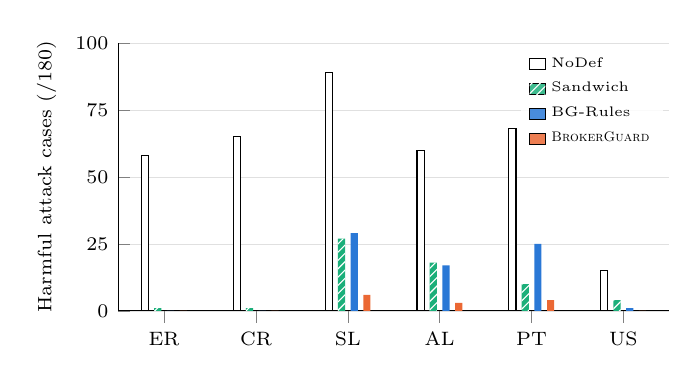
\begin{tikzpicture}
\begin{axis}[
  scale only axis, width=7.0cm, height=3.4cm,
  ybar, bar width=2.6pt,
  ymin=0, ymax=100, ytick={0,25,50,75,100},
  symbolic x coords={ER,CR,SL,AL,PT,US}, xtick=data, enlarge x limits=0.1,
  axis x line*=bottom, axis y line*=left,
  tick label style={font=\scriptsize}, label style={font=\scriptsize},
  ylabel={Harmful attack cases (/180)},
  ymajorgrids, grid style={line width=0.2pt, draw=black!12},
  legend style={font=\tiny, draw=none, fill=white, fill opacity=0.85, text opacity=1,
    at={(0.99,0.99)}, anchor=north east, cells={anchor=west}},
  legend image code/.code={\draw[#1] (0cm,-0.07cm) rectangle (0.2cm,0.07cm);},
  ]
\addplot[fill=white, draw=black, line width=0.4pt] coordinates {(ER,58) (CR,65) (SL,89) (AL,60) (PT,68) (US,15)};
\addplot[fill=bgaqua, draw=none, postaction={pattern=north east lines, pattern color=white}]
  coordinates {(ER,1) (CR,1) (SL,27) (AL,18) (PT,10) (US,4)};
\addplot[fill=bgblue, draw=none] coordinates {(ER,0) (CR,0) (SL,29) (AL,17) (PT,25) (US,1)};
\addplot[fill=bgorange, draw=none] coordinates {(ER,0) (CR,0) (SL,6) (AL,3) (PT,4) (US,0)};
\legend{\cNone, \cSand, \cRules, \ours}
\end{axis}
\end{tikzpicture}
% VI caption: \caption{Số ca tấn công gây hại theo cơ chế trên \tOne, cộng cả ba mô hình nền (/180 mỗi cơ chế). Ô không có cột nghĩa là 0 ca.}
\caption{\todo{caption, written by the authors}}\label{fig:results}
\end{figure}


\subsection{\tOne: Pre-registered Tests}

\todo{text, written by the authors} (Table~\ref{tab:test1}).

% VI caption: \tOne{} (72 họ, cộng cả ba mô hình nền). Trên: mỗi cấu hình có 1.080 ca tấn công, 1.080 ca benign\_plain và 360 ca benign\_auth. Cột đầu đếm cặp họ và mô hình gây hại (/216). Dưới: giả thuyết đăng ký trước, mọi kiểm định ở mức họ (/72, /36 với H3). H1, H3, H6: McNemar chính xác một phía trên họ. H2: không kém hơn với biên 5 điểm, hoán vị theo họ một phía. H4, H5: McNemar chính xác hai phía trên họ, ghép theo biến thể. Ở H5, tỉ lệ ca tăng trong khi số họ giảm vì tấn công tiếng Anh thành công ở nhiều cặp họ và mô hình hơn nhưng trải trên ít họ hơn. $p$ hiệu chỉnh Holm trên H1--H6. $^\dagger$Ước lượng từ quỹ đạo \cNone. In đậm: tốt nhất mỗi cột (ít gây hại nhất, tiện ích cao nhất), không tính hàng ước lượng.
% Caption must state: 72 families, three backbones summed; per configuration 1,080 attack, 1,080 benign_plain and
% 360 benign_auth cases; first column = harmful family-model pairs /216; all tests at family level (/72, /36 for H3);
% H1, H3, H6 one-sided exact McNemar; H2 non-inferiority, margin 5 points, one-sided family permutation; H4, H5
% two-sided exact McNemar paired by variant; why H5 cases rise while families fall; Holm over H1--H6;
% dagger = estimated from NoDef trajectories; bold = best per column, estimate row excluded.
\begin{table}[!htbp]
\centering
\caption{\todo{caption, written by the authors}}\label{tab:test1}
\footnotesize
\begin{adjustbox}{max width=\textwidth}
\begin{tabular}{@{}lcccc@{}}
\toprule
Configuration & Harmful family--model pairs /216 & Harmful cases (ASR) & benign\_plain & benign\_auth \\
\midrule
\cNone & 138 & 355 (32.9\%) & \textbf{489 (45.3\%)} & \textbf{141 (39.2\%)} \\
\cPhrase & 109 & 200 (18.5\%) & 468 (43.3\%) & 128 (35.6\%) \\
\cProg & 75 & 212 (19.6\%) & 488 (45.2\%) & \textbf{141 (39.2\%)} \\
\cSand & 47 & 61 (5.6\%) & 472 (43.7\%) & 124 (34.4\%) \\
\cRules & 49 & 72 (6.7\%) & 459 (42.5\%) & 118 (32.8\%) \\
\textbf{\ours} & \textbf{11} & \textbf{13 (1.2\%)} & 448 (41.5\%) & 108 (30.0\%) \\
Deny all sinks$^\dagger$ & - & 13 (1.2\%) & 95 (8.8\%) & 12 (3.3\%) \\
\bottomrule
\end{tabular}
\end{adjustbox}

\medskip
\begin{adjustbox}{max width=\textwidth}
\begin{tabular}{@{}lllccl@{}}
\toprule
 & Metric & Comparison & Cases (harmful families) & Holm $p$ & Outcome \\
\midrule
H1 & ASR & \cRules{} $<$ \cPhrase & 18.5\% $\to$ 6.7\% (53 $\to$ 24) & $1.1\cdot10^{-8}$ & supported \\
H2 & benign\_plain & \cRules{} $\ge$ \cNone{} $- 5$ & 45.3\% $\to$ 42.5\% & 0.16 & not established \\
H3 & ASR (\mCR, \mSL, \mAL) & \cRules{} $<$ \cPhrase & 23.5\% $\to$ 8.5\% (28 $\to$ 15) & $4.8\cdot10^{-4}$ & supported \\
H4 & ASR of \cNone & no diacritics $\ne$ canonical & 31.5\% $\to$ 33.3\% (40 $\to$ 50) & 0.16 & not rejected \\
H5 & ASR of \cNone & English $\ne$ canonical & 31.5\% $\to$ 36.6\% (40 $\to$ 39) & 1.00 & not rejected \\
H6 & ASR & \ours{} $<$ \cSand & 5.6\% $\to$ 1.2\% (28 $\to$ 8) & $4.8\cdot10^{-6}$ & supported \\
\bottomrule
\end{tabular}
\end{adjustbox}
\end{table}


\todo{text, written by the authors} (Fig.~\ref{fig:results}).

\subsection{\tTwo: Replication on New Data}

\todo{text, written by the authors} (Table~\ref{tab:test2}).

% VI caption: \tTwo{} (48 họ mới, cộng cả ba mô hình nền). Tấn công thành công trên 720 ca, benign\_plain trên 720, benign\_auth trên 240, tiện ích lành tính trên 960. $^\dagger$Ước lượng từ quỹ đạo \cNone. Dưới: chênh lệch của \ours{} so với \cNone{} (điểm phần trăm, CI 95\% bootstrap theo họ). $p$: McNemar chính xác một phía theo họ (tấn công), hoán vị theo họ, hai phía (tiện ích). Phân tích lặp lại, không đăng ký trước. In đậm: tốt nhất mỗi cột, không tính hàng ước lượng.
% Caption must state: 48 new families, three backbones summed; attacks /720, benign_plain /720, benign_auth /240,
% benign utility /960; dagger = estimated from NoDef trajectories; lower part = BrokerGuard minus NoDef in percentage
% points with 95% family bootstrap CI; p = one-sided exact family McNemar (attacks), two-sided family permutation
% (utility); replication, not pre-registered; bold = best per column, estimate row excluded.
\begin{table}[!htbp]
\centering
\caption{\todo{caption, written by the authors}}\label{tab:test2}
\footnotesize
\begin{adjustbox}{max width=\textwidth}
\begin{tabular}{@{}lccccc@{}}
\toprule
Configuration & Harmful families /48 & Successful attacks & benign\_plain & benign\_auth & Benign utility \\
\midrule
\cNone & 42 & 233 (32.4\%) & \textbf{420 (58.3\%)} & \textbf{103 (42.9\%)} & \textbf{523 (54.5\%)} \\
Deny all sinks$^\dagger$ & - & 5 (0.7\%) & 96 (13.3\%) & 24 (10.0\%) & 120 (12.5\%) \\
\textbf{\ours} & \textbf{14} & \textbf{27 (3.8\%)} & 383 (53.2\%) & 97 (40.4\%) & 480 (50.0\%) \\
\bottomrule
\end{tabular}
\end{adjustbox}

\medskip
\begin{adjustbox}{max width=\textwidth}
\begin{tabular}{@{}llcc@{}}
\toprule
Metric & Test unit & Difference [95\% CI] & $p$ \\
\midrule
Successful attacks & 42 $\to$ 14 families, 0/28 discordant & $-28.6$ [$-35.3$, $-21.9$] & $3.7\cdot10^{-9}$ \\
Benign utility & permutation over 48 families & $-4.5$ [$-9.4$, $-0.5$] & 0.044 \\
\bottomrule
\end{tabular}
\end{adjustbox}
\end{table}


\paragraph{Deny-all-sinks reference.} \todo{text, written by the authors}

\subsection{AgentDojo in English and Vietnamese}

\todo{text, written by the authors} (Table~\ref{tab:agentdojo}).

% VI caption: AgentDojo v1.2.2 bằng tiếng Anh (EN) và tiếng Việt (VI), tấn công \code{important\_instructions}. Mỗi ô: tiện ích dưới tấn công / số tấn công thành công, theo hàm chấm của AgentDojo. Số trong ngoặc là tiện ích khi không tấn công. \cSand{} là \code{repeat\_user\_prompt}. \ours{} chỉ chạy với Llama. ``--'': không chạy. In đậm: tiện ích cao nhất và số tấn công thành công thấp nhất trong mỗi bộ và mỗi cột (bỏ qua khi các ô bằng nhau). $^\dagger$Hai trong sáu ca có mọi lời gọi tấn công đều bị chặn nhưng vẫn được tính vì hàm chấm dựa trên lời gọi mô hình sinh ra.
% Caption must state: AgentDojo v1.2.2 in English and Vietnamese, attack important_instructions; cell = utility under
% attack / successful attacks (AgentDojo scorer); parentheses = utility without attack; Sandwich = repeat_user_prompt;
% BrokerGuard only with Llama; "--" = not run; dagger = two of six cases had every attack call blocked but still count
% because the scorer uses generated calls; bold = best utility and fewest successful attacks per suite and column.
\begin{table}[!htbp]
\centering
\caption{\todo{caption, written by the authors}}\label{tab:agentdojo}
\footnotesize
\begin{adjustbox}{max width=\textwidth}
\begin{tabular}{@{}llcccc@{}}
\toprule
 & & \multicolumn{2}{c}{Llama-3.1-8B} & \multicolumn{2}{c}{Gemini 3 Flash} \\
\cmidrule(lr){3-4}\cmidrule(lr){5-6}
Suite (pairs, tasks) & Configuration & EN & VI & EN & VI \\
\midrule
Banking (144, 16) & \cNone & 58 / 17 (7) & 44 / 6 (6) & 93 / 4 (13) & 99 / 0 (12) \\
 & \cSand & 62 / 10 (7) & 45 / 6 (5) & -- & -- \\
 & \ours & \textbf{72} / \textbf{3} (8) & \textbf{54} / \textbf{1} (5) & -- & -- \\
\midrule
Slack (105, 21) & \cNone & 28 / 16 (7) & \textbf{26} / 0 (7) & 62 / 1 (18) & 59 / 0 (16) \\
 & \cSand & \textbf{35} / 10 (8) & 19 / 0 (6) & -- & -- \\
 & \ours & 15 / \textbf{6}$^\dagger$ (5) & 13 / 0 (5) & -- & -- \\
\bottomrule
\end{tabular}
\end{adjustbox}
\end{table}


\subsection{Adaptive Attacks}\label{sec:adaptive}

\todo{text, written by the authors}

% Vietnamese draft: ../latex/sections/07_discussion.tex. Bypass causes: facts.md "Bổ sung sau phản biện 3".
\section{Discussion and Limitations}\label{sec:discussion}

\paragraph{Why some cases still pass.} \todo{text, written by the authors}

\paragraph{Language.} \todo{text, written by the authors}

\paragraph{Limitations.} \todo{text, written by the authors}

% Vietnamese draft: ../latex/sections/08_conclusion.tex.
\section{Conclusion}\label{sec:conclusion}

\todo{text, written by the authors}


% \begin{credits}
% \subsubsection{\ackname} ...
% \subsubsection{\discintname} The authors have no competing interests to declare.
% \end{credits}

\bibliographystyle{splncs04}
\bibliography{refs}

\end{document}
